\chapter{Hadronic Recoil Corrections}\label{ch:recoil}

Missing transverse energy spectra of the W and Z signal simulation does not fully describe the observed distributions in data. This is attributable to multiple effects, such as mis-modeling of multiple scattering and detector simulation, or imperfect detector calibration in data. Therefore, the simulated \met spectrum is not able to describe the observed \met spectrum to sufficient precision necessary for this measurement. Corrections to the hadronic recoil in simulated events in W and Z events are used to match the data and MC \met resolution and response. 

The W and Z share a similar production mechanism and are similar in mass, so data corrections derived from \zmm. The hadronic recoil of each event is corrected, and the \met is recomputed based on these corrected values. 

The hadronic recoil is characterized as the negative vector sum of the \met and the \pt of the daughter leptons from the W or Z, as shown in Equation~\ref{eq:ch10:recoil}. This is effectively everything "else" in the event except for the W and daughter leptons.
\begin{equation}
\vec{U}=-(\vec{E_T^{miss}}+\sum{p_{T}^l})
    % \caption{}
    \label{eq:ch10:recoil}
\end{equation}

The recoil is split into two components: the projection parallel to the boson momentum, \upar, and perpendicular to the boson momentum, $u_\perp$, as shown in Equations~\ref{eq:ch10:upar} and~\ref{eq:ch10:uprp}. 
\begin{equation}
    u_{||} = \vec{U}\cdot \vec{Z_{p_T}}
    \label{eq:ch10:upar}
\end{equation}

\begin{equation}
    u_\perp = \vec{U} -  u_{||}
    \label{eq:ch10:uprp}
\end{equation}


The \upar and \uprp observables are both the source and target of the recoil corrections. The method by which these distributions are parametrized and corrected are described in the following sections.

%% Also get a figure for this section, probably the vector diagram of the recoils


%%%%%%%%%%%%%%%%%%%%%%%%%%%%%%%%%%%%%%%%%
%%%%%%%%%%%    modeling
%%%%%%%%%%%%%%%%%%%%%%%%%%%%%%%%%%%%%%%%%

\section{Recoil Modeling} \label{ch:recoil:modeling}
the goal of recoil corrections is to derive a map to transform a source distribution of recoil values onto a target distribution of recoil values to provide an accurate Monte Carlo prediction of the MET spectrum. In this case, the source is the Z->ll or Wlnu Monte Carlo, and the target is data. Recoil components are parametrized for 3 samples: data, Z MC, and W MC. To apply recoil corrections to the Z sample, one only needs to replace the Z MC recoil distributions with those of Z data. Correction on the W requires an additional intermediate step of correcting to the Z Monte Carlo recoil before correcting to the Z data recoil.

\section{Parametrization Derivation}
Recoil is parametrized in generally the same way for each of the samples:
\begin{enumerate}
\item \upar and \uprp are binned by boson \pt
\item \upar and \uprp  in each \pt bin are fit with a double-Gaussian function
\end{enumerate}
Figures~\ref{fig:recoil:data_fit_example}
 and ~\ref{fig:recoil:mc_fit_example} provide examples of these double-Gaussian fits in data and simulation. Recoil parametrization is done in data for \zmm and simulation for \zmm and \wmunu. The reference boson \pt for the Z is from the reconstructed dilepton system $\mu_1+\mu_2$. For W events, the boson \pt is directly from the generator-level information in the simulation. These corrections are further separated by charge, to be applied separately to $W^+$ and $W^-$.
Additionally, fits for \upar and \uprp in Z data include the simulated dilepton background contributions from electroweak and \ttbar sources.

\begin{figure}
\centering
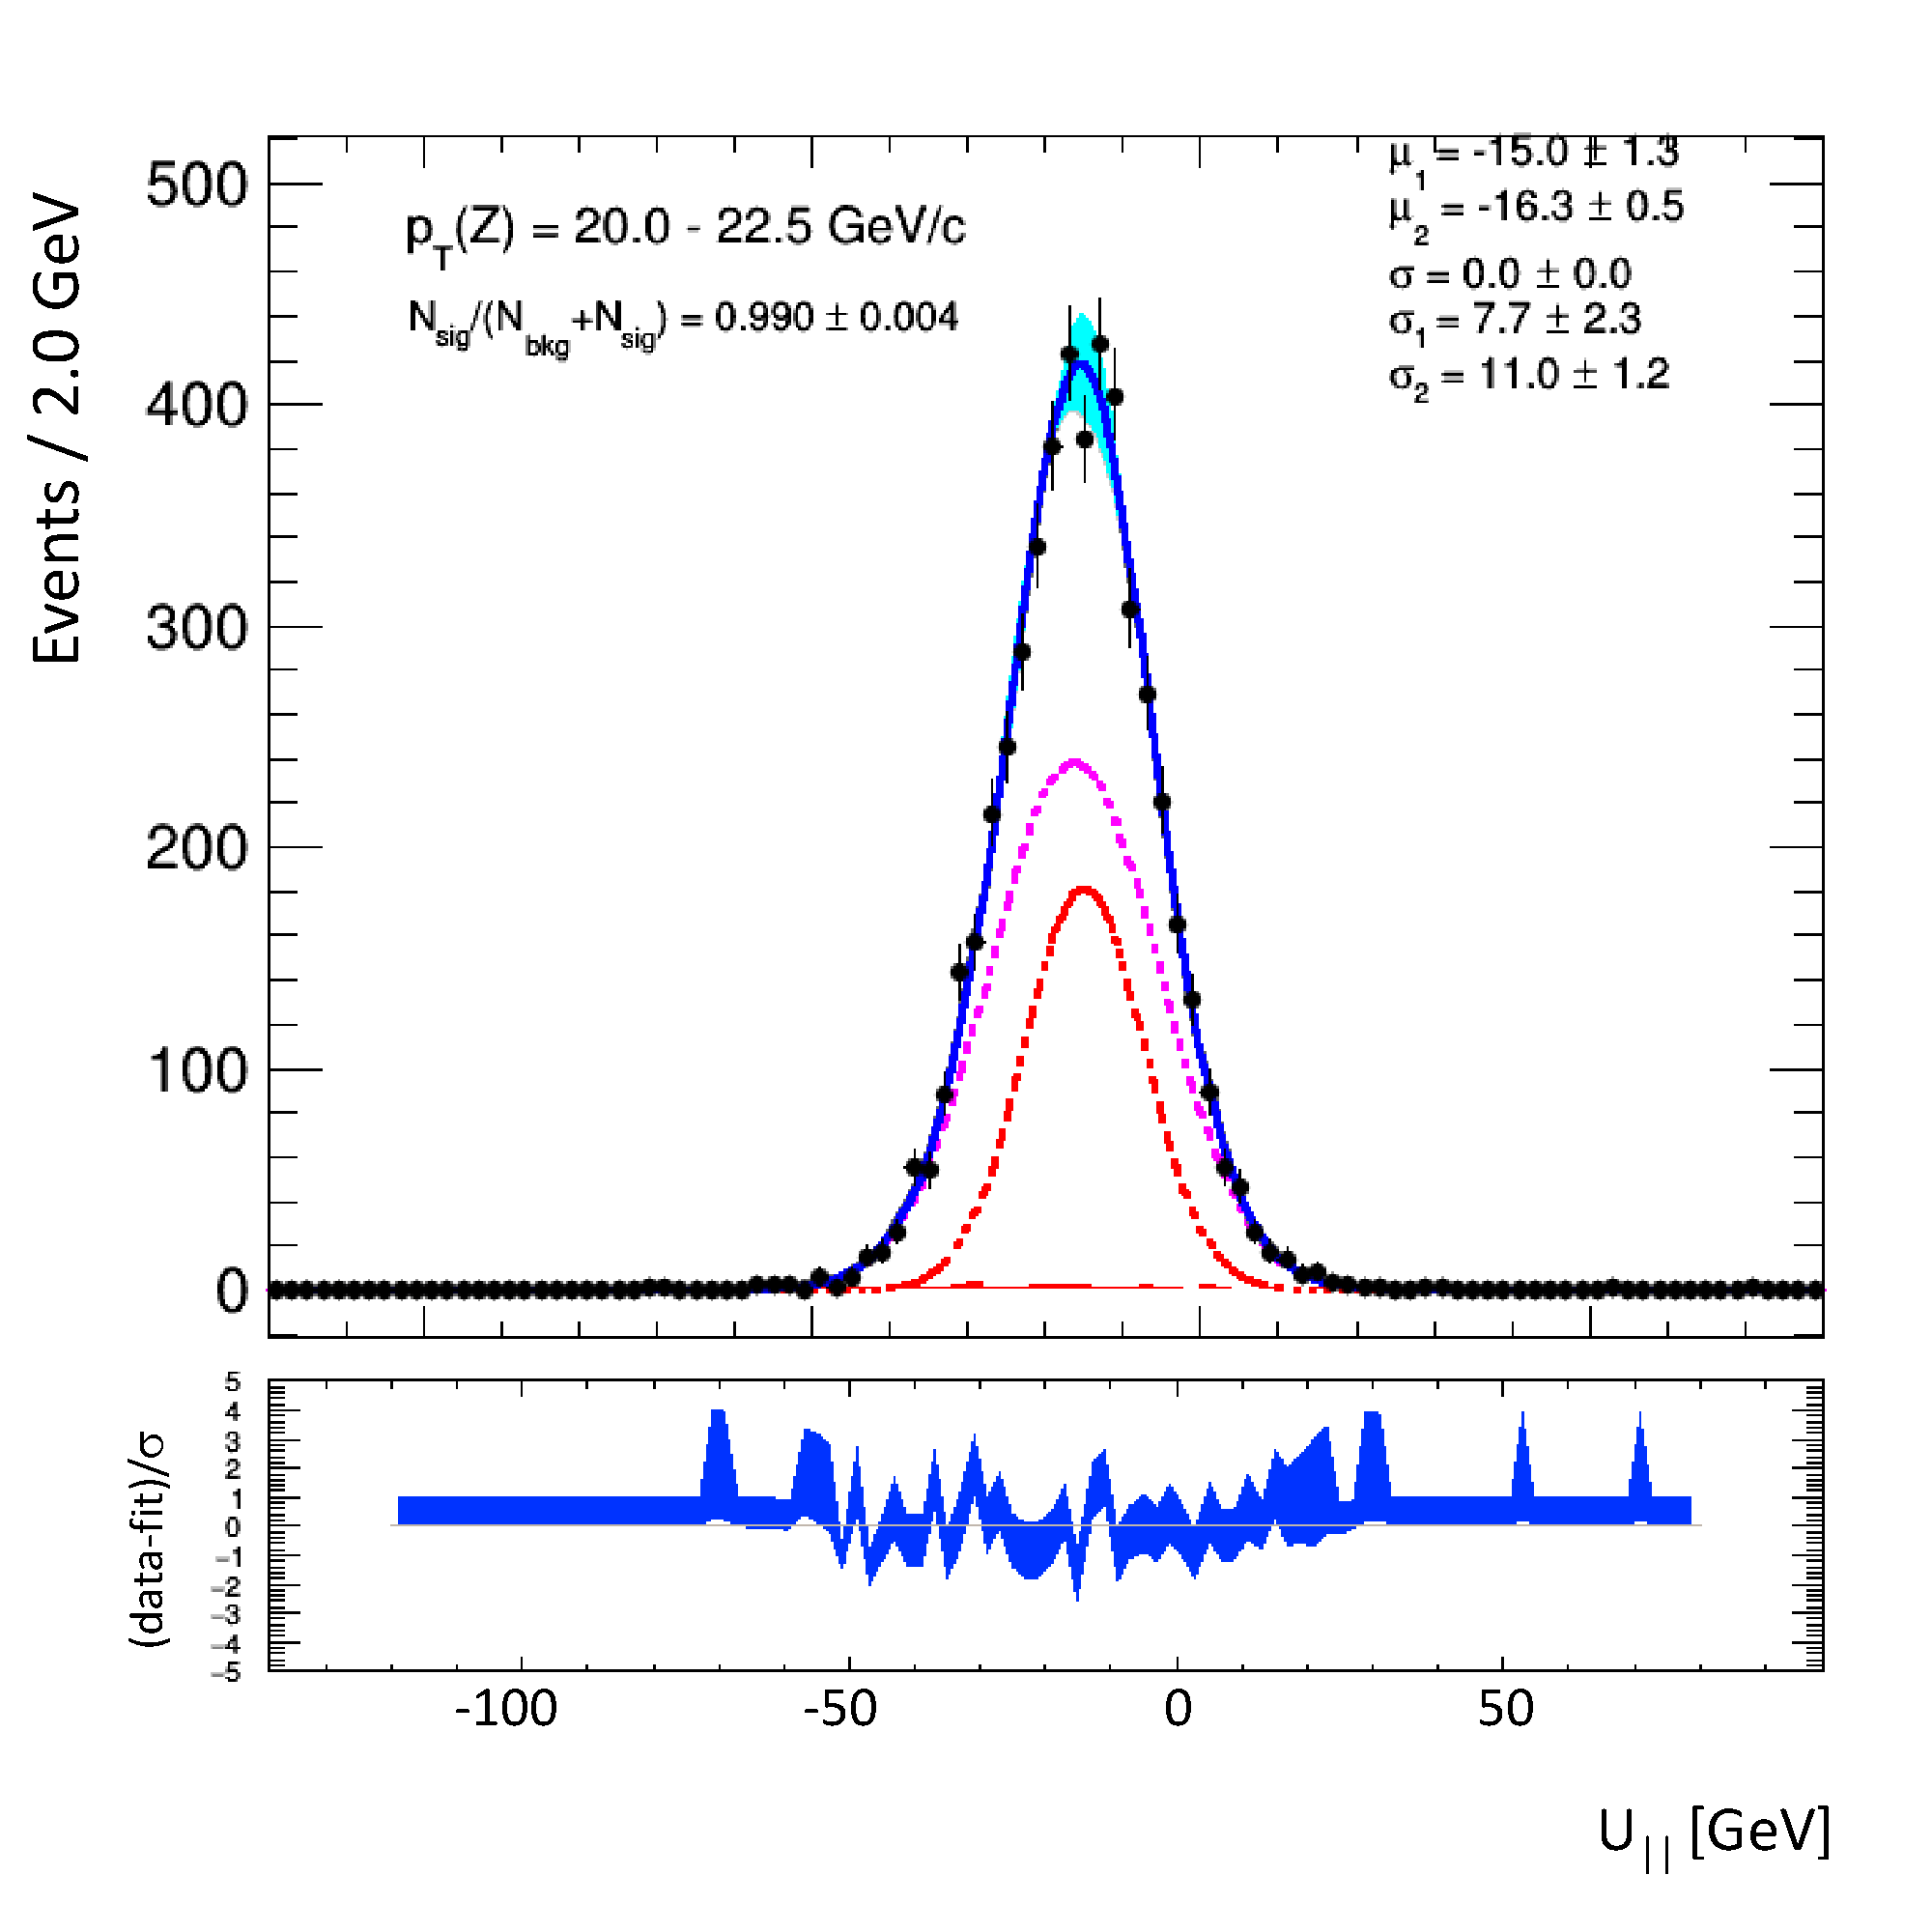
\includegraphics[width=0.49\linewidth]{plots/Recoil/example-data-pfu1fit_12.pdf}
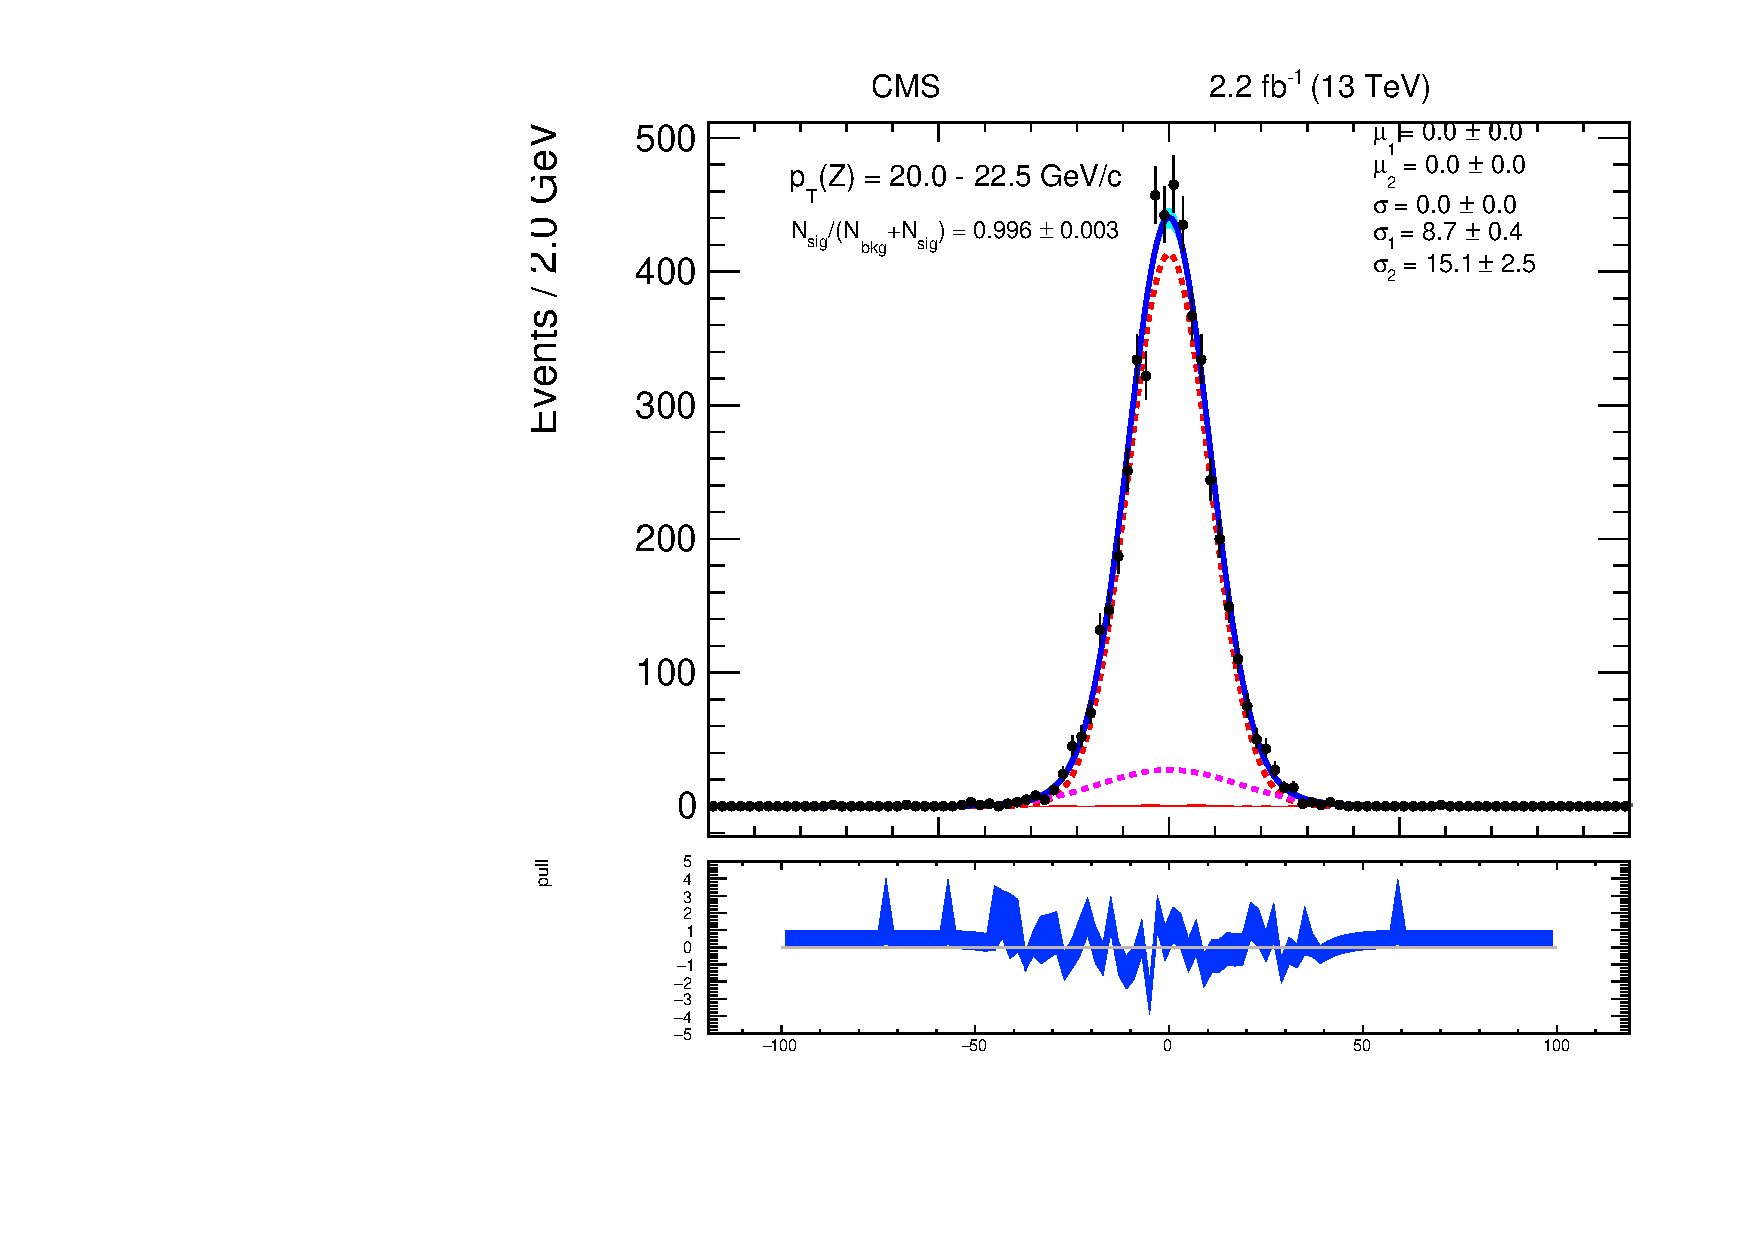
\includegraphics[width=0.49\linewidth]{plots/Recoil/example-data-pfu2fit_12.pdf}
\caption{Examples of the recoil parametrization fits in data for $20~\mathrm{GeV} < m_{\mu\mu}  < 22.5~\mathrm{GeV}$. The two Gaussians are shown, with their sum in blue.}
\label{fig:recoil:data_fit_example}
\end{figure}
\begin{figure}
\centering
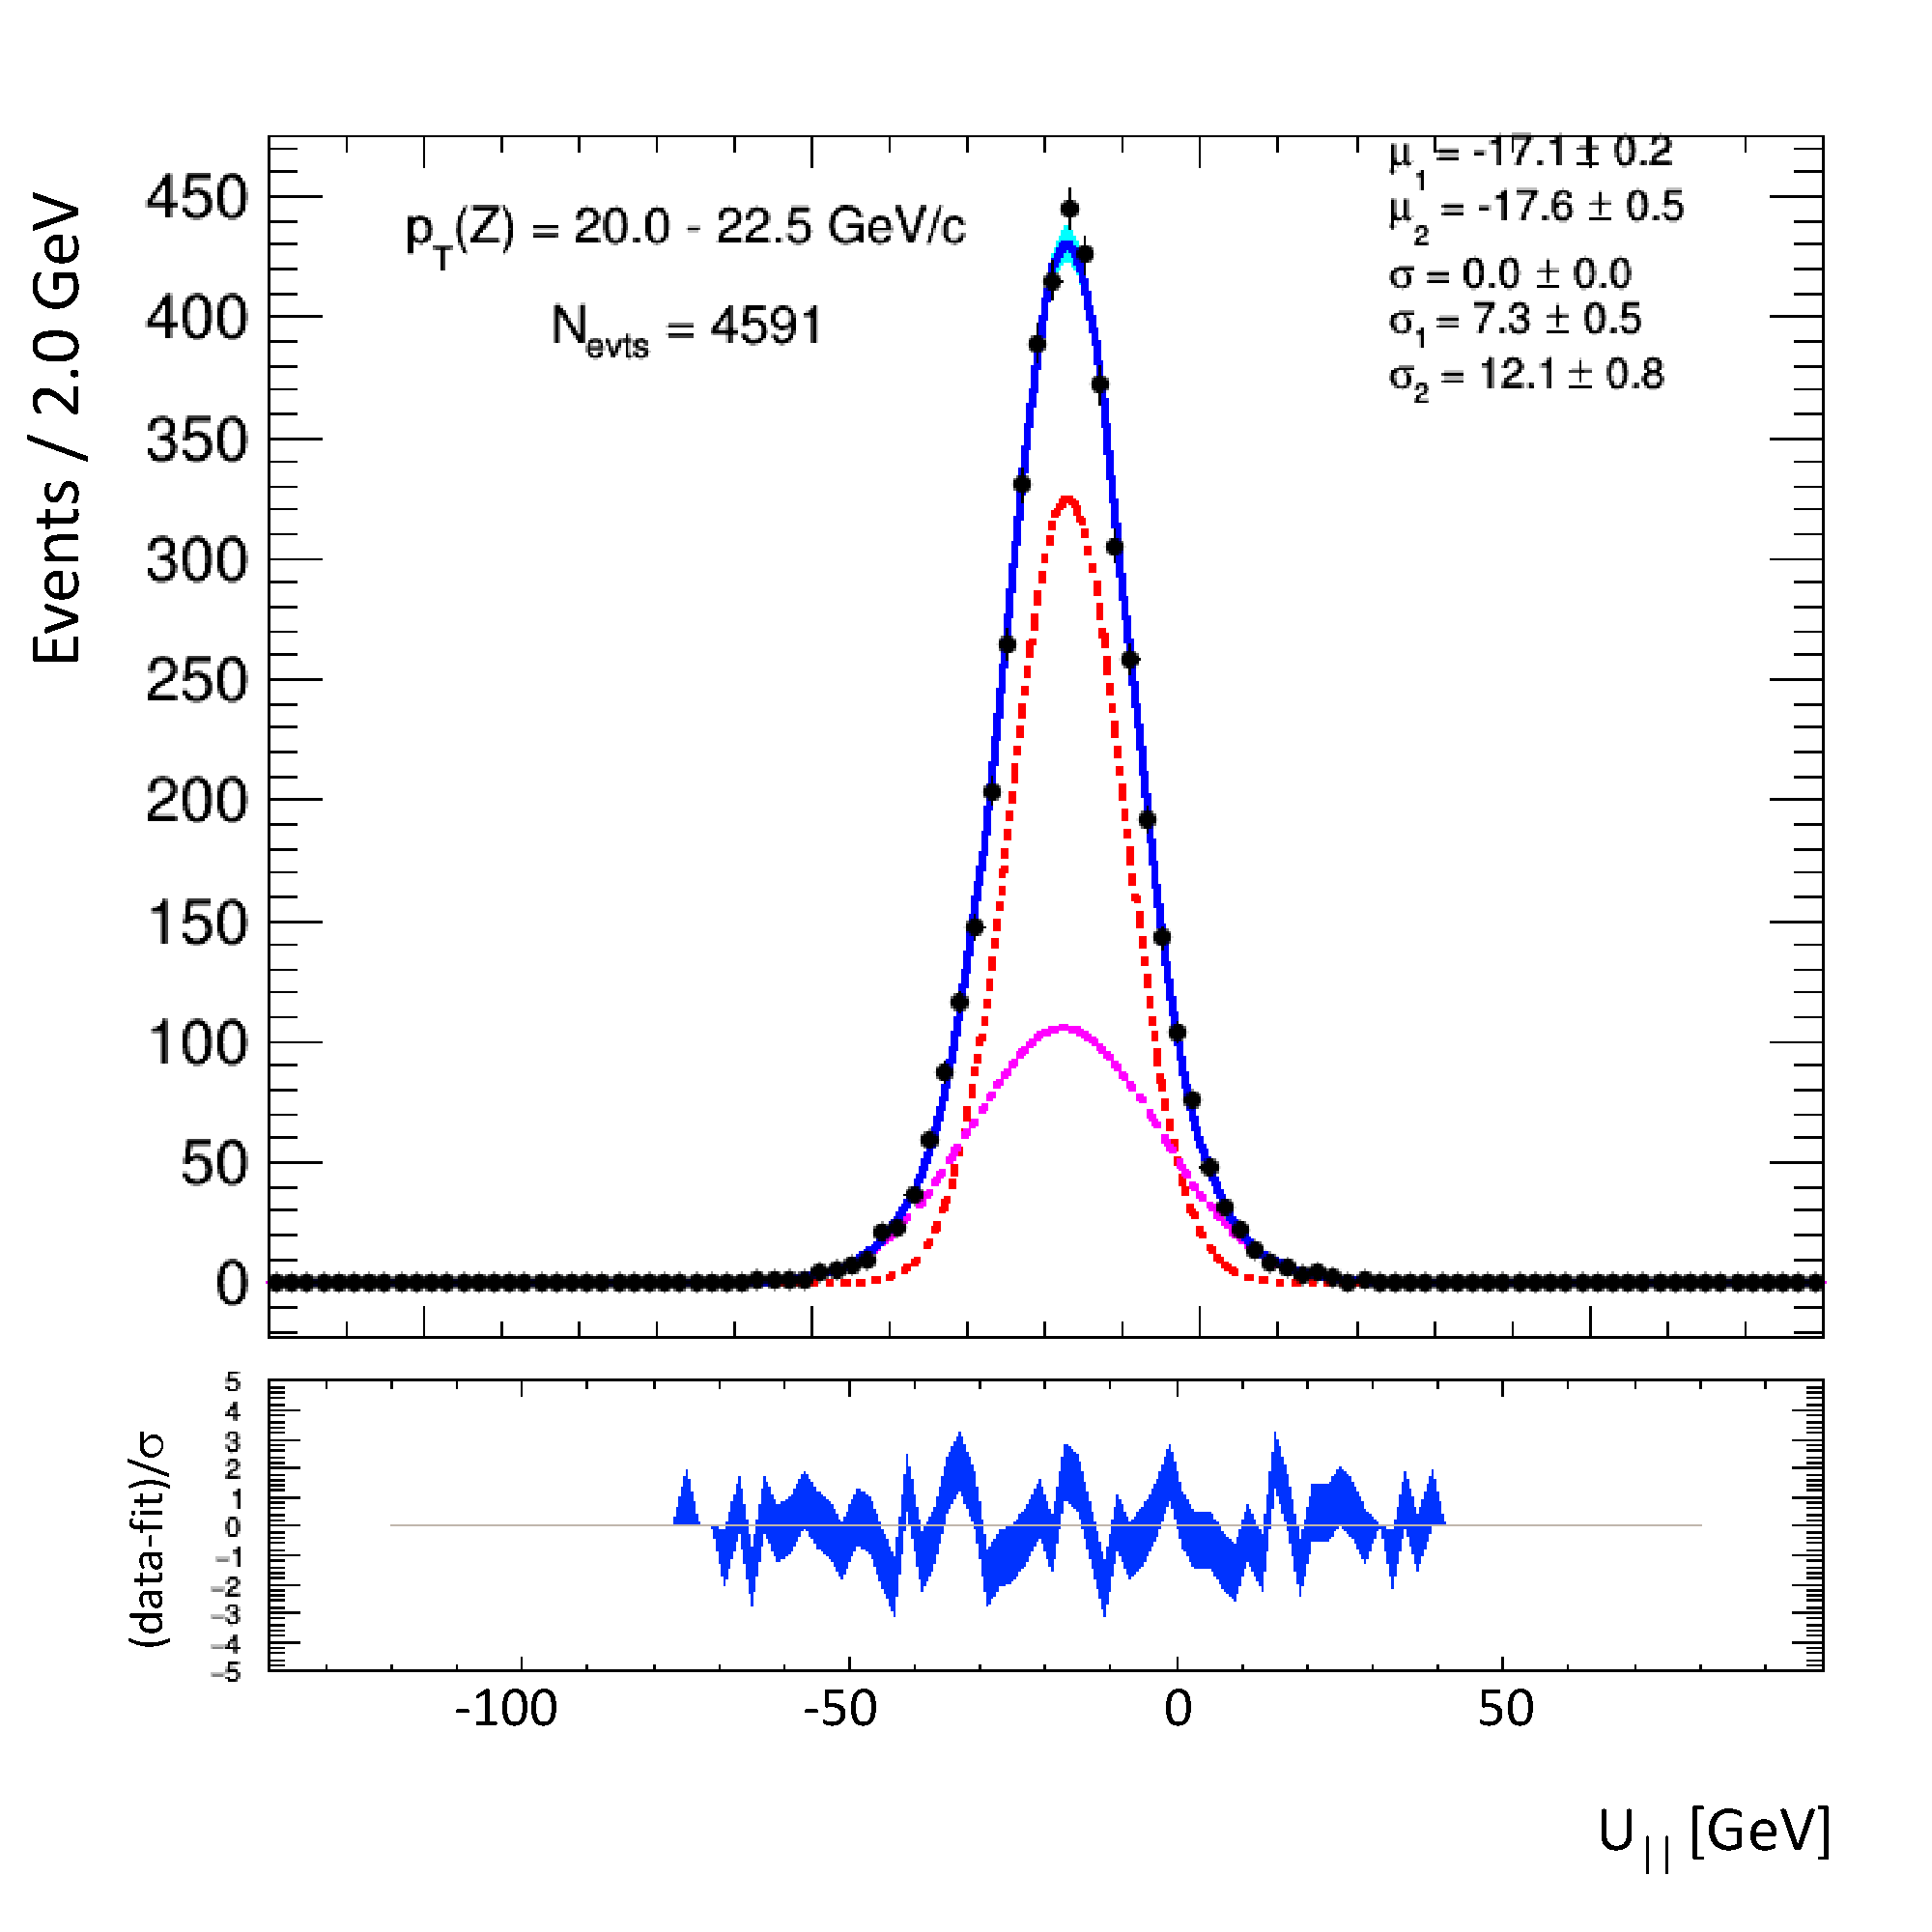
\includegraphics[width=0.49\linewidth]{plots/Recoil/example-mc-pfu1fit_12.pdf}
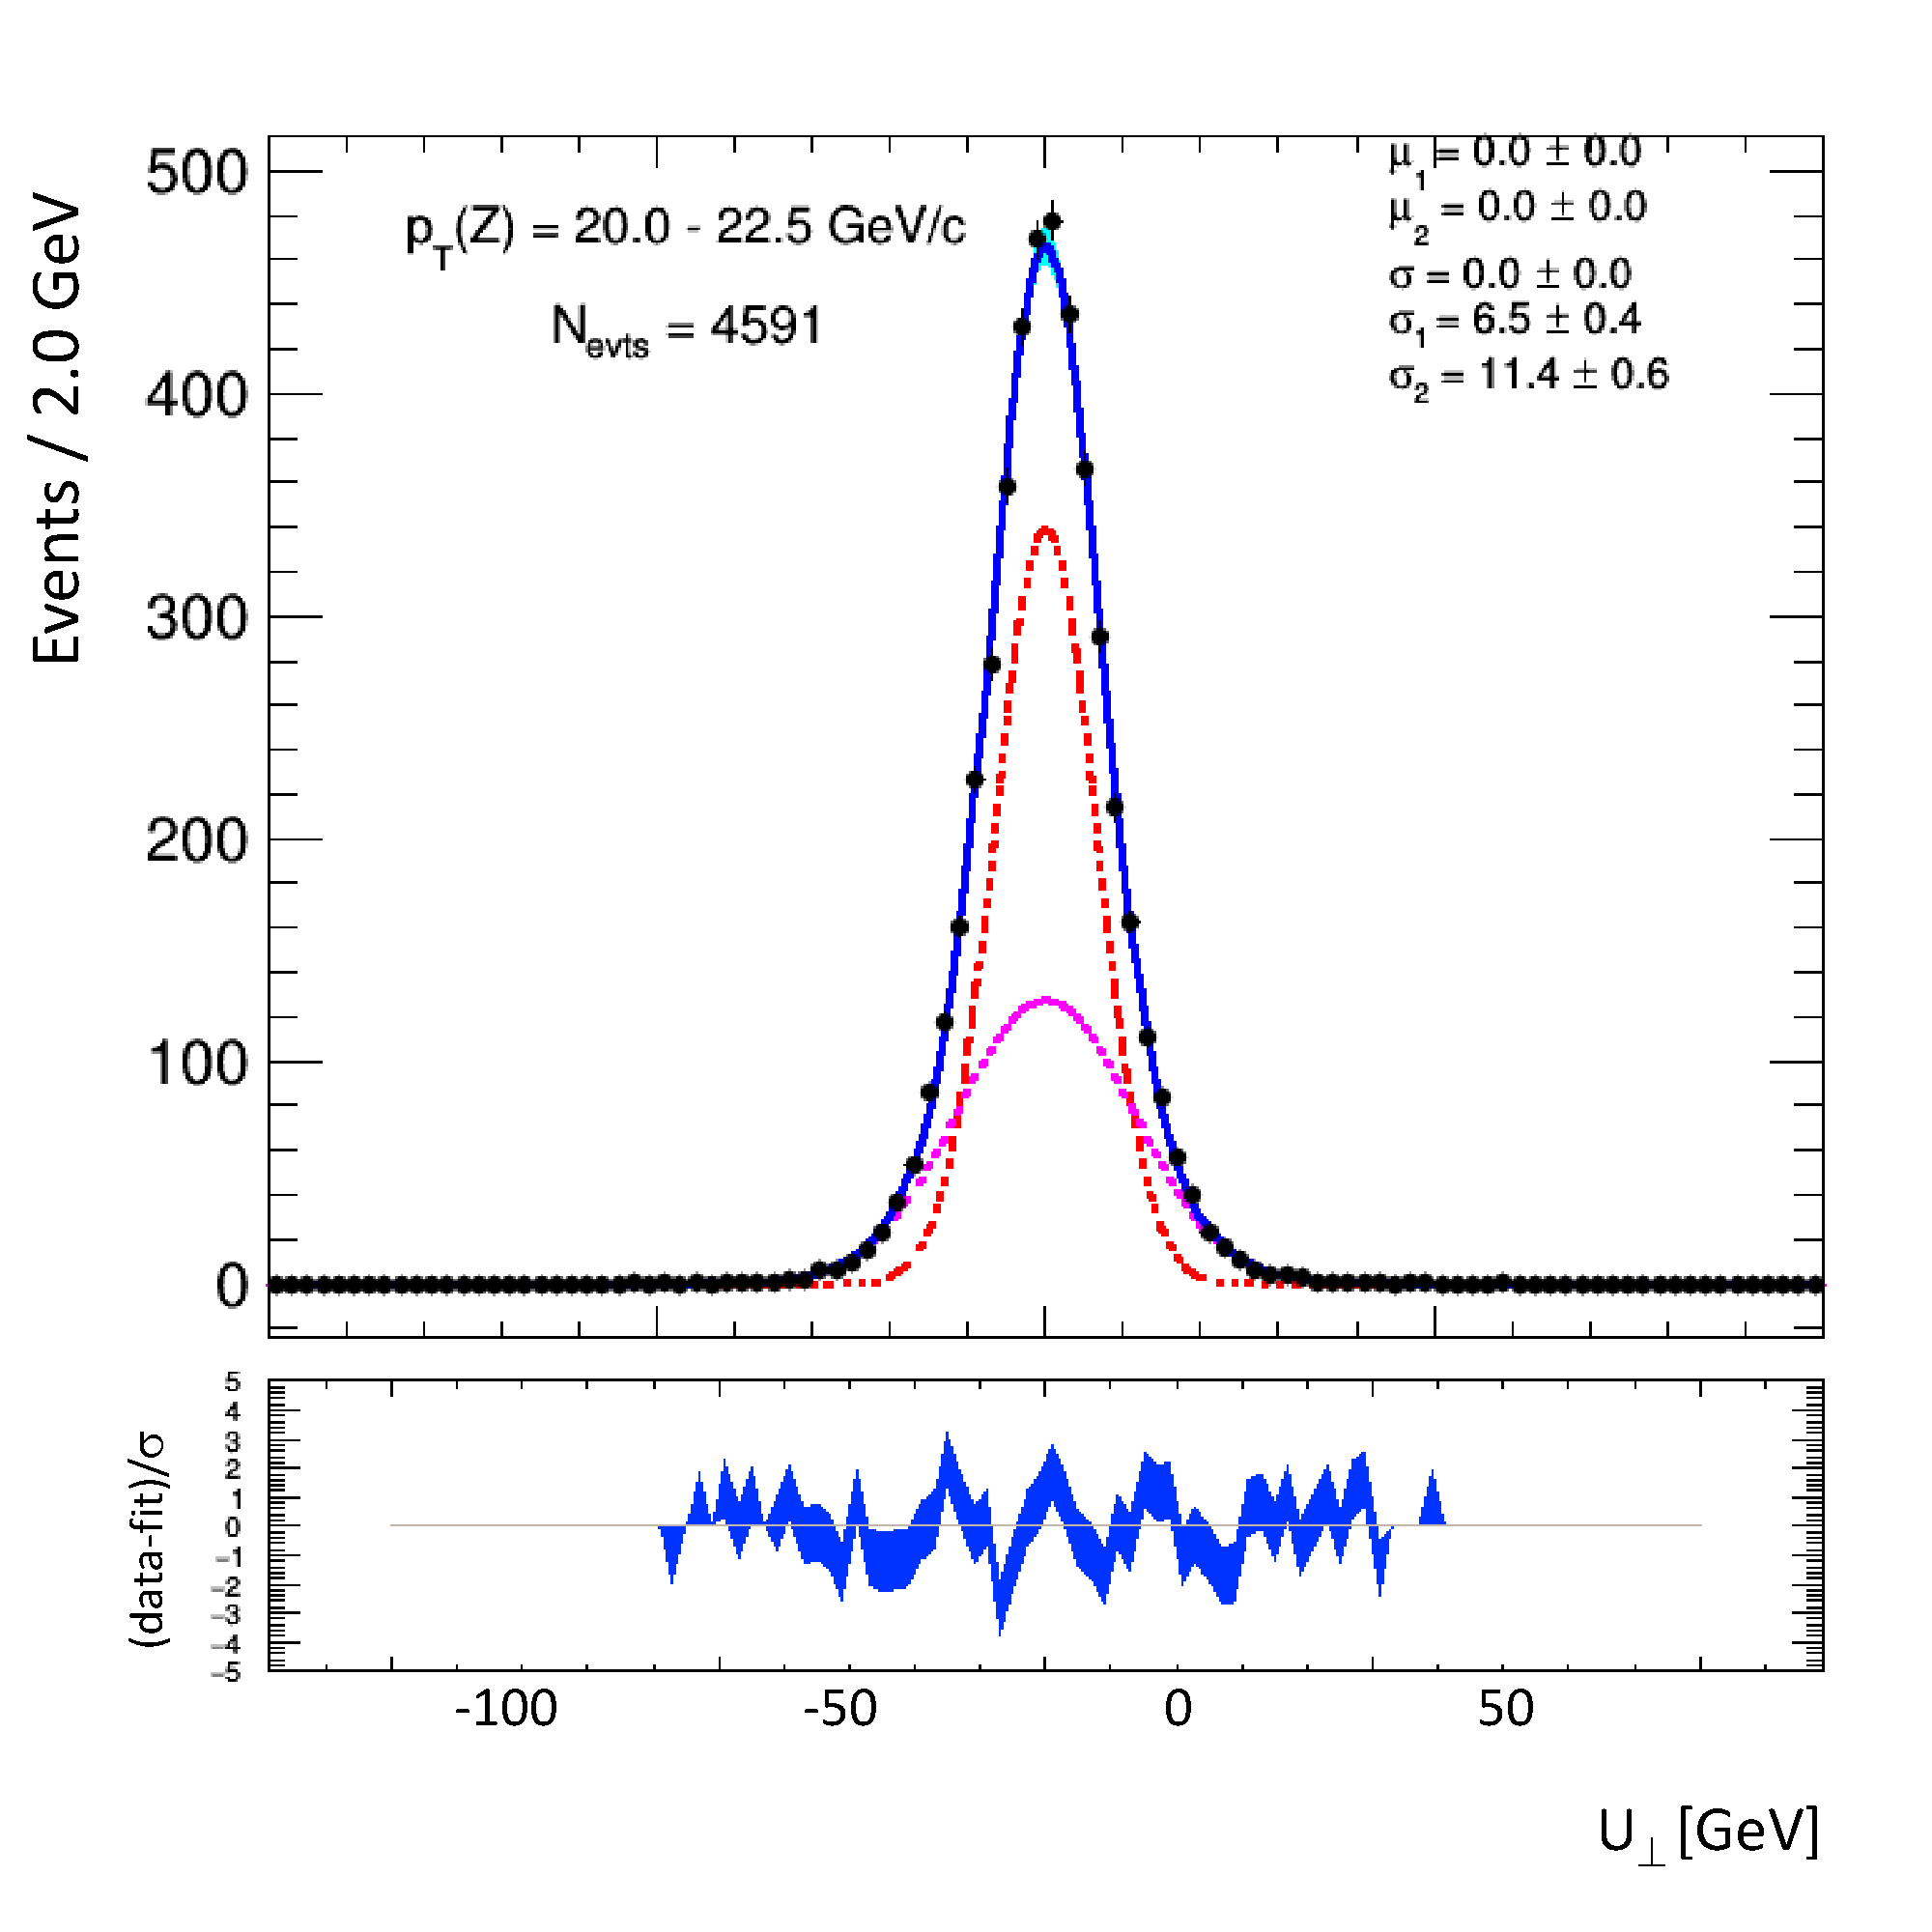
\includegraphics[width=0.49\linewidth]{plots/Recoil/example-mc-pfu2fit_12.pdf}
\caption{Examples of the recoil parametrization fits for $u_{||}$ (left) and $u_{\perp}$ (right) in MC for $20~\mathrm{GeV} < m_{\mu\mu}  < 22.5~\mathrm{GeV}$. The two Gaussians are shown, with their sum in blue.}
\label{fig:recoil:mc_fit_example}
\end{figure}

%%%%%%%%%%%%%%%%%%%%%%%%%%%%%%%%%%%%%%%%%
%%%%%%%%%%%    application
%%%%%%%%%%%%%%%%%%%%%%%%%%%%%%%%%%%%%%%%%

% put in a couple of plots
\section{Application of Corrections}\label{ch:recoil:apply}
The corrections derived in the previous section can be applied to the \W or \Z Monte Carlo. For simulated \W or \Z event, the original \upar and \uprp are replaced by a corrected value and the \met is recomputed. 
\subsubsection{CDF inversion method} \label{ch10:recoil:apply}
Using the same boson \pt definition that was used to create the parametrization, the recoil distributions for MC are corrected to match data via a CDF inversion into the data recoil distribution: 
\begin{enumerate}
    \item Each fit result is integrated to create a cumulative distribution function
    \item A p-value is determined by evaluating the W CDF from MC: $p_{i}=F_{U_{i}}^{M}(u_{i})$
    \item A coreccted $u_i^{M}$ value is determined by finding the root of the Z MC CDF at $p$: $u_{i}^{M}={F_{U_{i}}^{Data}}^{-1}(p_{i})$
    \item A p-value is determined by evaluating the W CDF from MC: $p_{i}=F_{U_{i}}^{M}(u_{i})$
    \item A coreccted $u_i^{Data}$ value is determined by finding the root of the Z MC CDF at $p$: $u_{i}^{Data}={F_{U_{i}}^{Data}}^{-1}(p_{i})$
    \item The difference between the $u_i^D$ and $u_i^M$ is added to the original recoil component to created the corrected value:  $u_{i}' = u_{i} + (u_i^D - u_i^M) $
    \item $u_{||}'$ and $u_{\perp}'$ are used to compute a new MET value for the event
\end{enumerate}
In the case where recoil corrections are applied to the Z sample, the effective steps are reduced to  

\subsubsection{Validation}
The effect of the recoil corrections on the Zmm MET spectrum and recoil spectrum are shown in Figures~\ref{fig:recoil:validation:met}~and~\ref{fig:recoil:validation:recoil}.

\begin{figure}
\centering
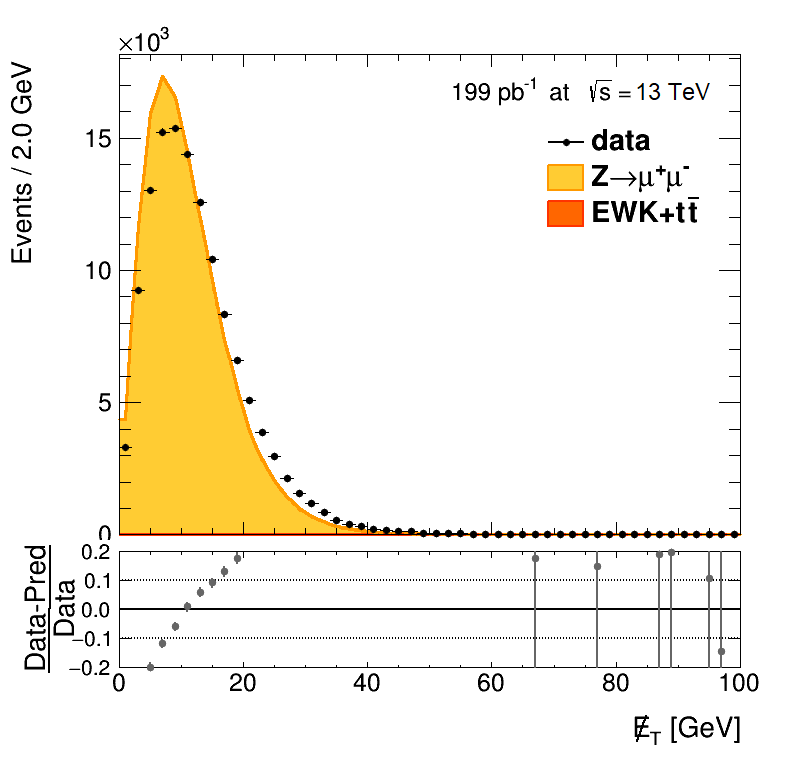
\includegraphics[width=0.49\linewidth]{plots/Recoil/close_nocorr_13/fitmetp.png}
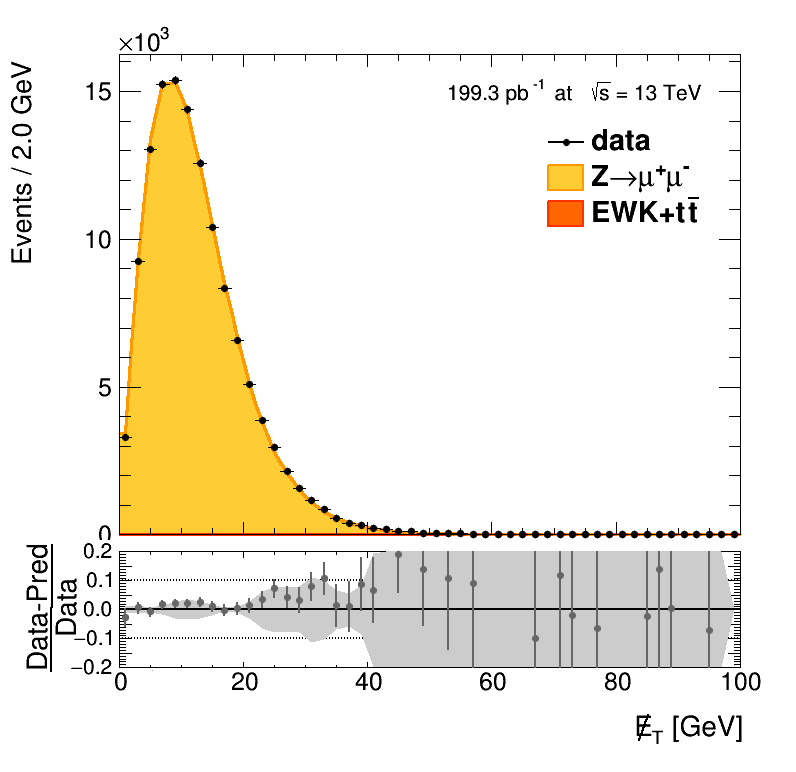
\includegraphics[width=0.49\linewidth]{plots/Recoil/close_corr_13/fitmetp.png}
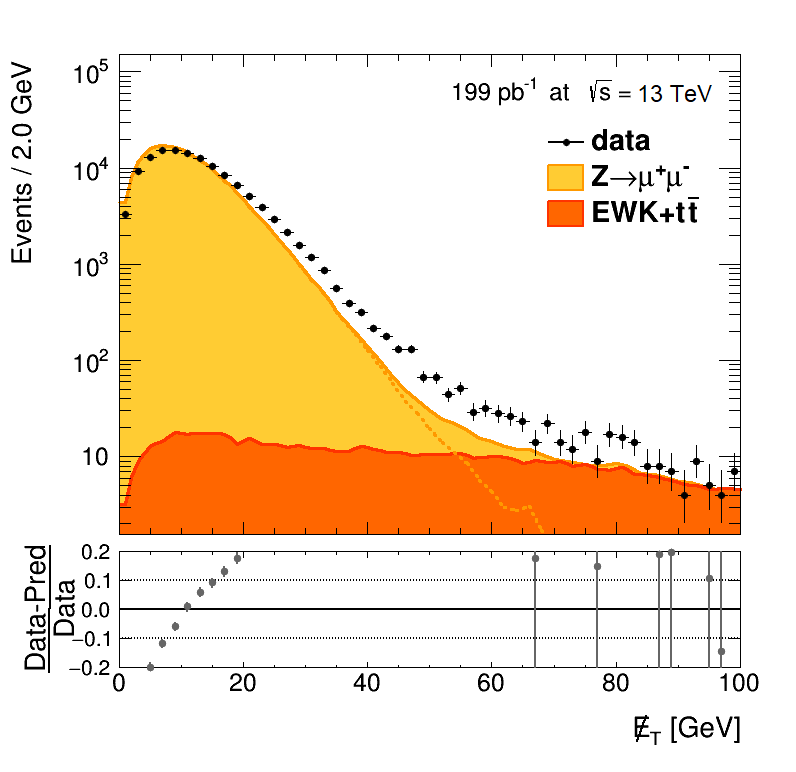
\includegraphics[width=0.49\linewidth]{plots/Recoil/close_nocorr_13/fitmetplog.png}
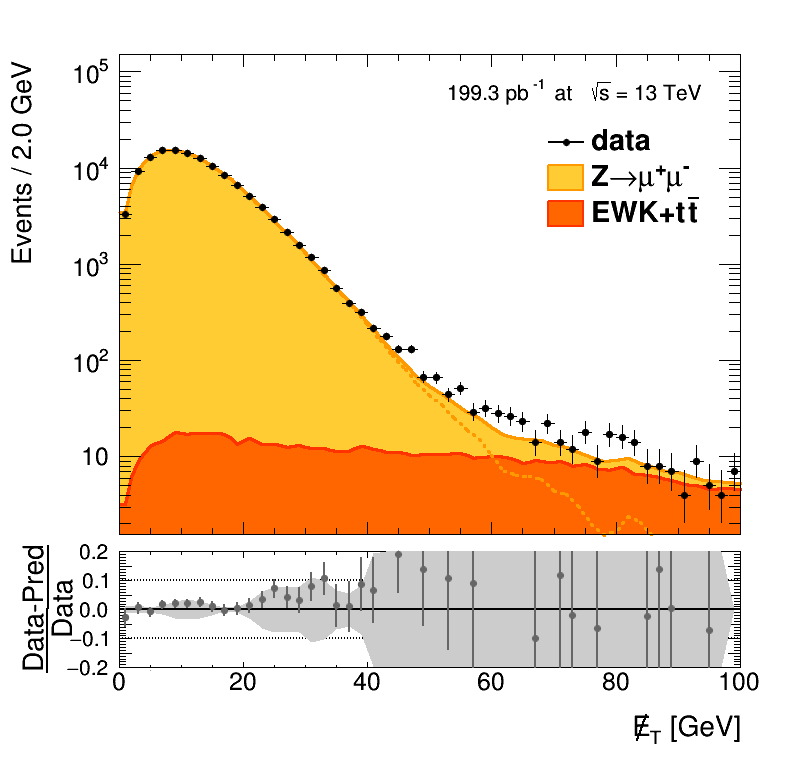
\includegraphics[width=0.49\linewidth]{plots/Recoil/close_corr_13/fitmetplog.png}
\caption{\met spectrum for \zmm sample, without (left) and  including (right) recoil corrections on linear (top) and log-y (bottom) scales. Gray band on recoil-corrected figures shows total uncertainty from modeling and statistical sources.}
\label{fig:recoil:validation:met}
\end{figure}
\begin{figure}
\centering
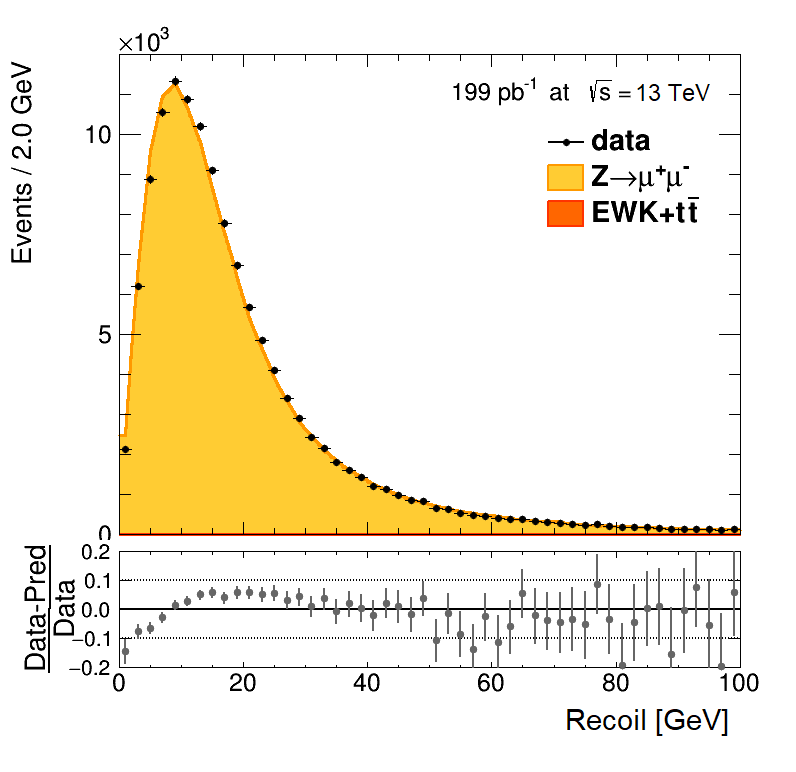
\includegraphics[width=0.49\linewidth]{plots/Recoil/close_nocorr_13/fitrecoilp.png}
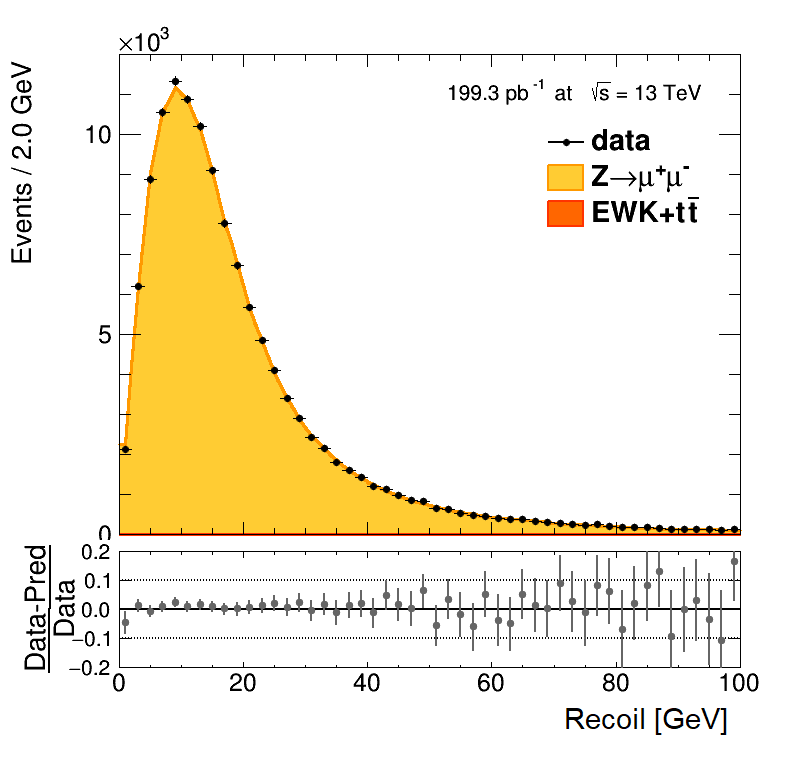
\includegraphics[width=0.49\linewidth]{plots/Recoil/close_corr_13/fitrecoilp.png}
\caption{Recoil spectrum for Zmm sample, pre- and post-recoil correction.}
\label{fig:recoil:validation:recoil}
\end{figure}

Closure of the recoil correction derivation is performed by comparing recoil against the Z in data to the pre- and post-correction recoil in Z Monte Carlo. A comparison between the pre-correction Z MC, post-correction Z MC, and data is shown in Figure~\ref{fig:recoil:validation:13} [13 TeV] and Figure~\ref{fig:recoil:validation:5} [5 TeV].


\begin{figure}
\centering
\begin{subfigure}{.50\textwidth}
\centering
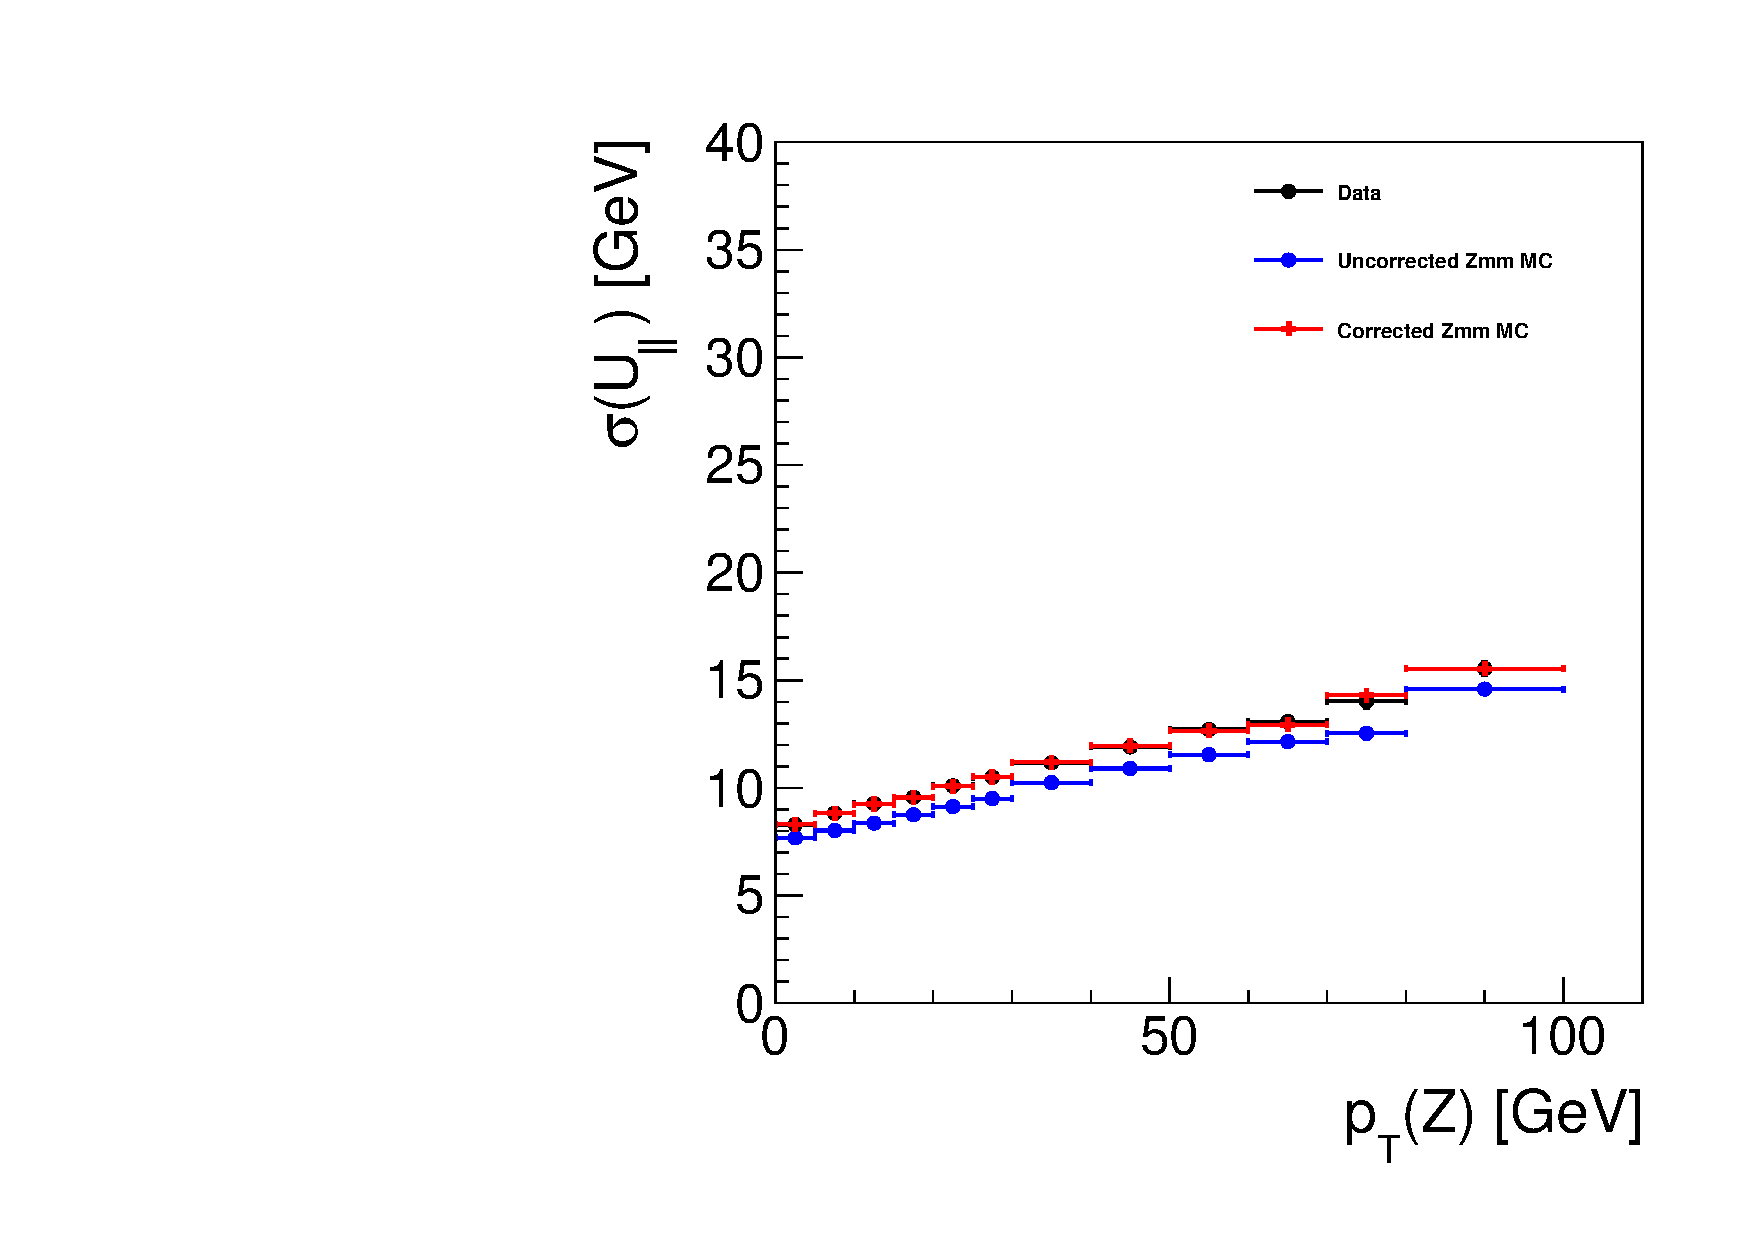
\includegraphics[width=\linewidth]{plots/Recoil/validation_13/resolution_par.pdf}
 \caption{Resolution of \upar}
%   \label{fig:Eff:el:5TeV:GSFSel:pos
\end{subfigure}%
\centering
\begin{subfigure}{.50\textwidth}
\centering
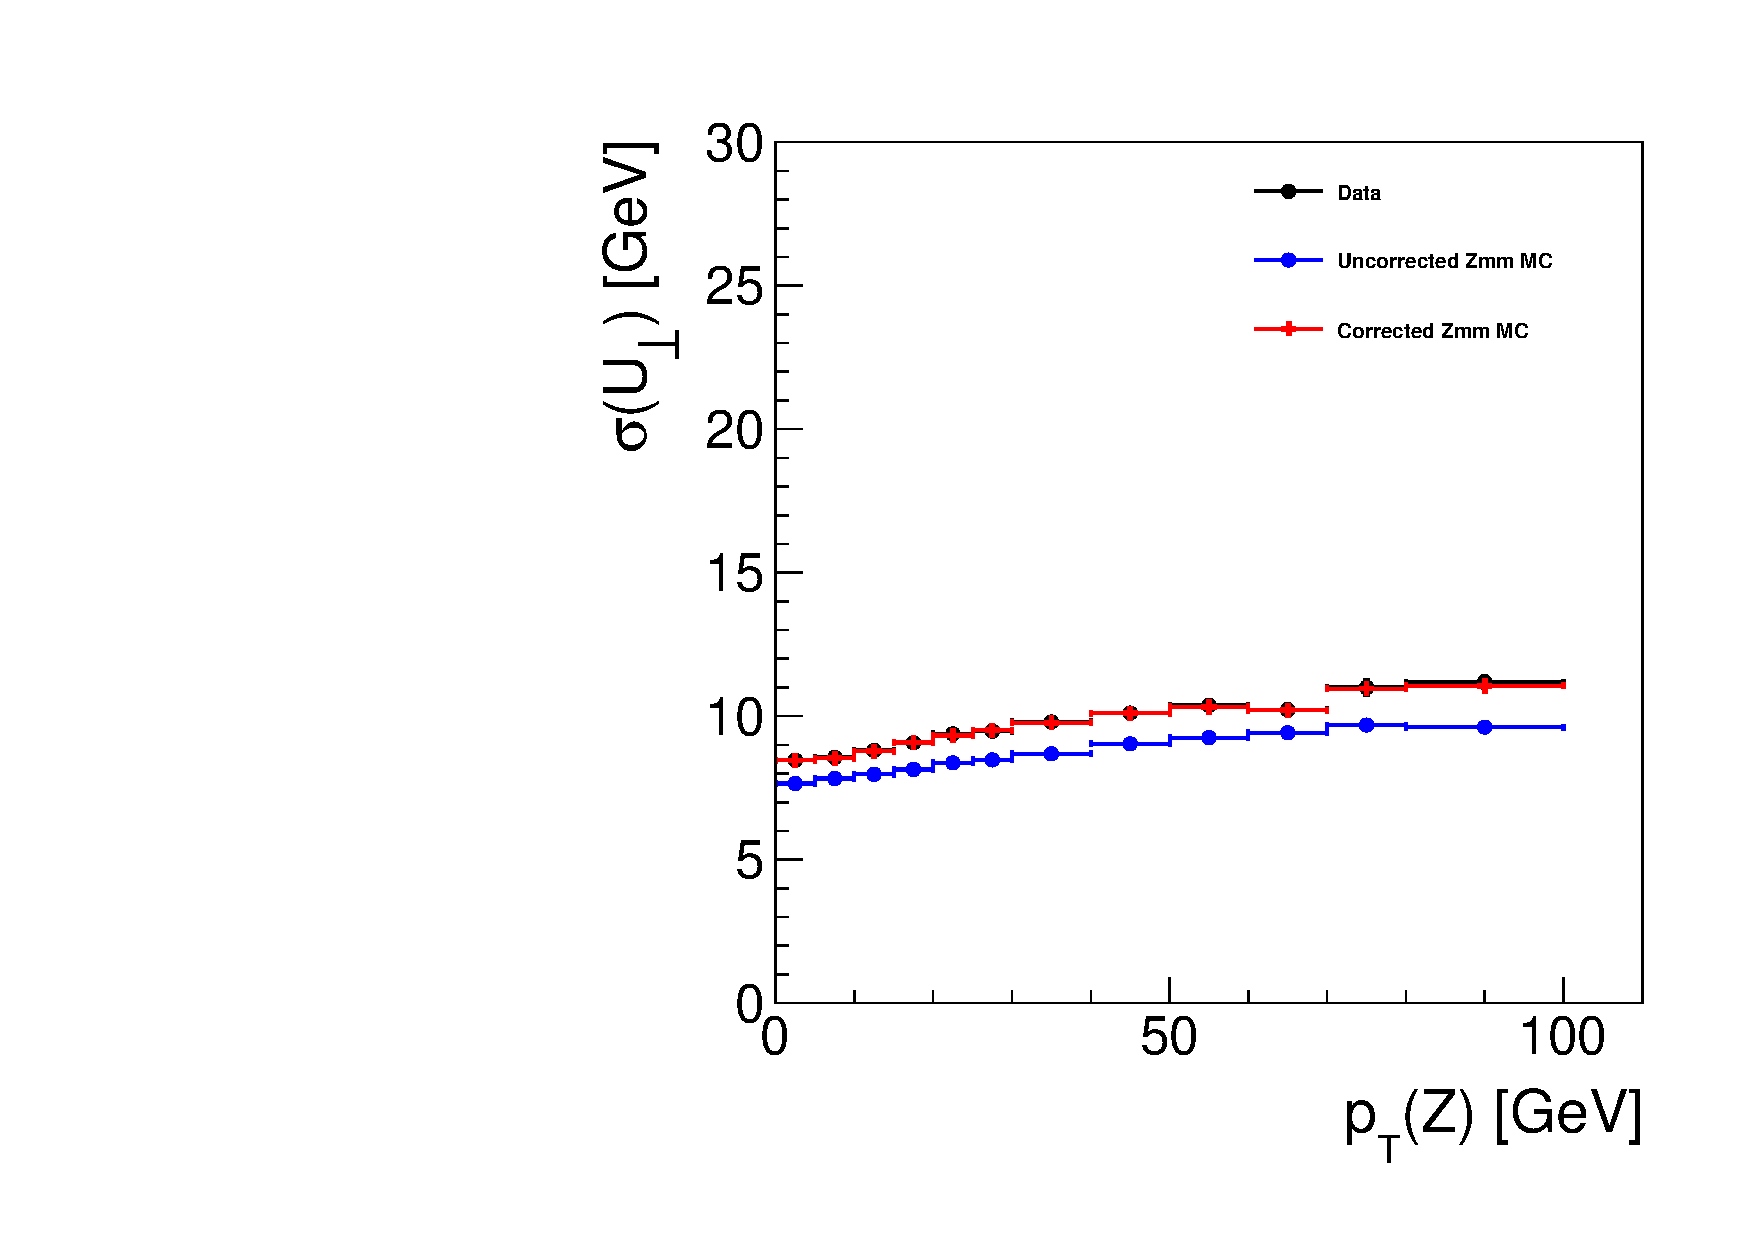
\includegraphics[width=\linewidth]{plots/Recoil/validation_13/resolution_prp.pdf}
\caption{Resolution of \uprp}
%   \caption{1a}
%   \label{fig:Eff:el:5TeV:GSFSel:pos
\end{subfigure}%
\\
\centering
\begin{subfigure}{.50\textwidth}
\centering
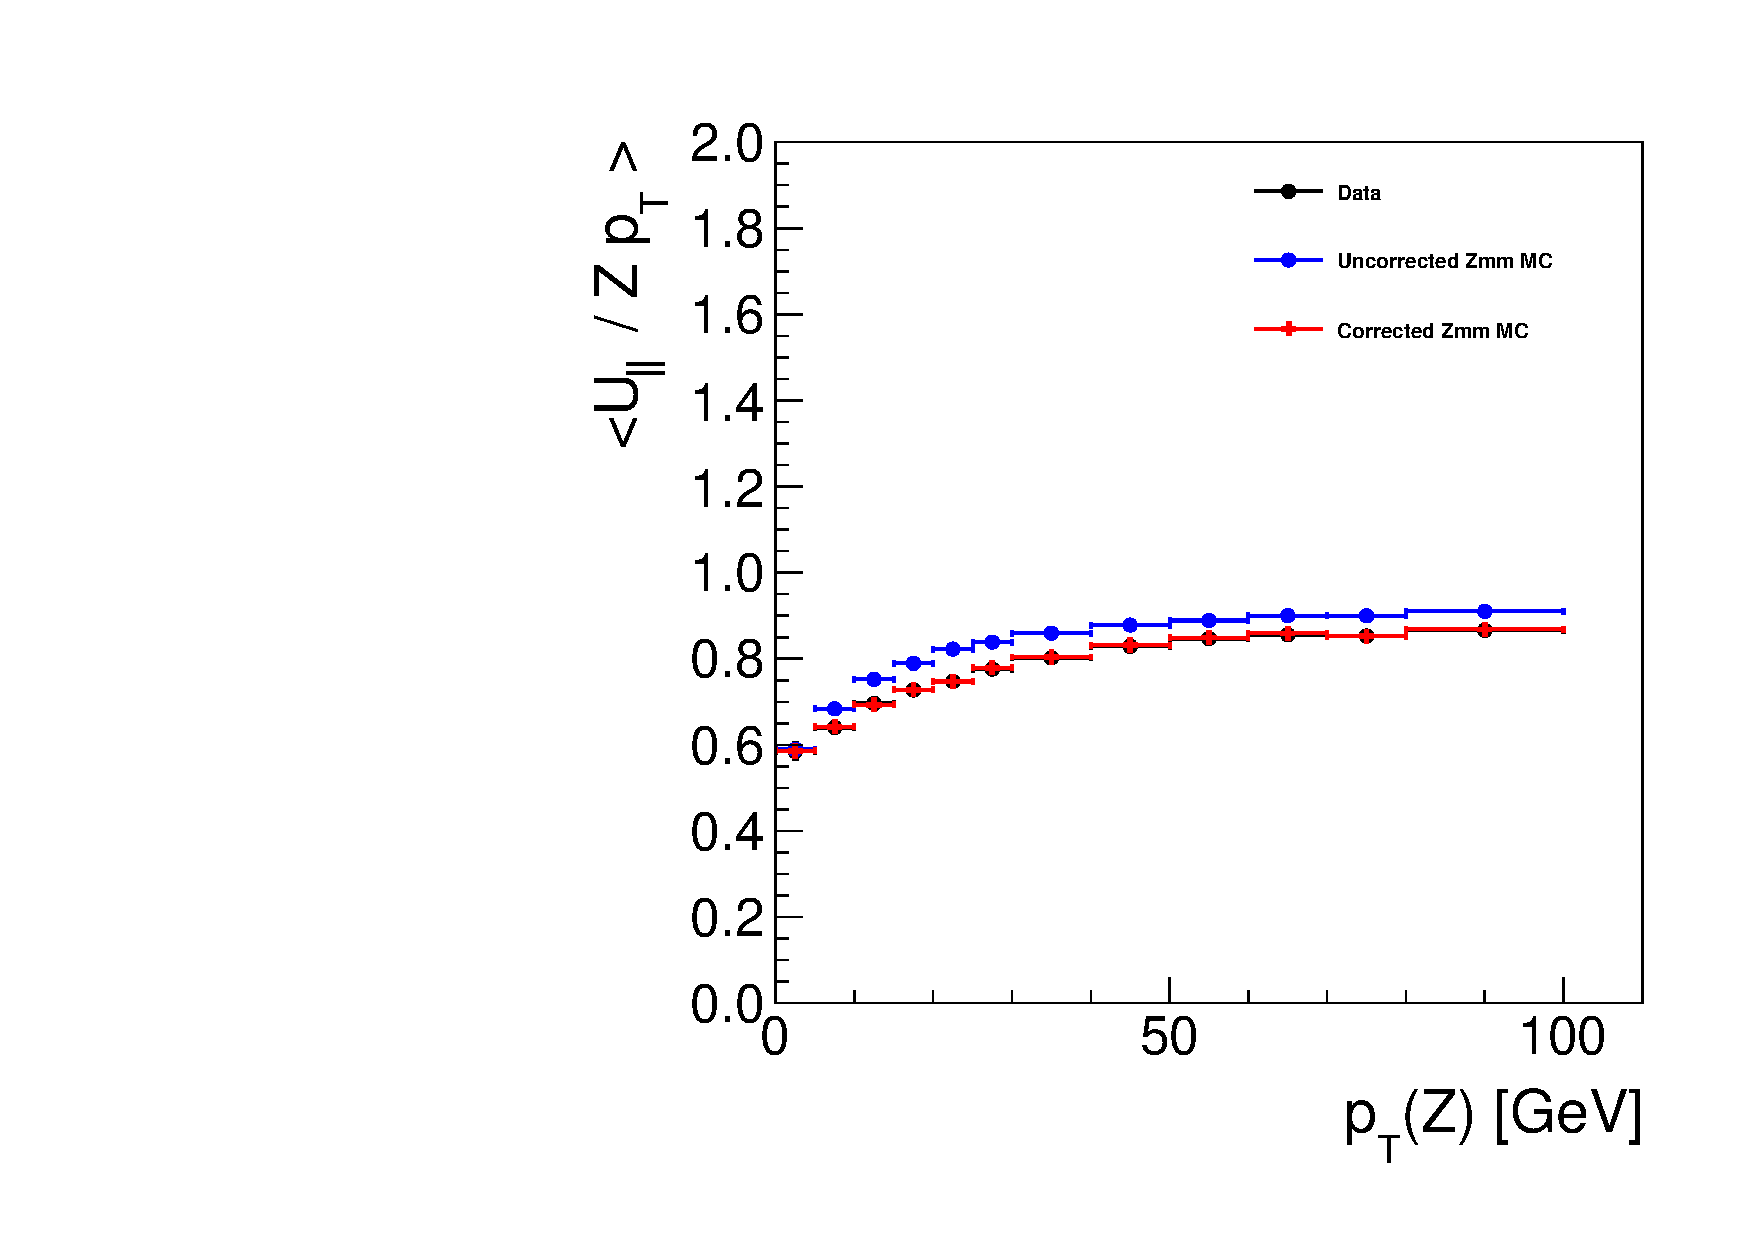
\includegraphics[width=\linewidth]{plots/Recoil/validation_13/response_par.pdf}
\caption{$p_T$-corrected response of \upar}
%   \caption{1a}
%   \label{fig:Eff:el:5TeV:GSFSel:pos
\end{subfigure}%
\caption{Closure of the recoil corrections derived from and applied to $Z\rightarrow\mu\mu$ samples for the 13 TeV dataset. The raw recoil distribution in Monte Carlo [blue] is corrected [red] towards the target spectrum of data [black].}
\label{fig:recoil:validation:13}
\end{figure}

\begin{figure}
\centering
\begin{subfigure}{.50\textwidth}
\centering
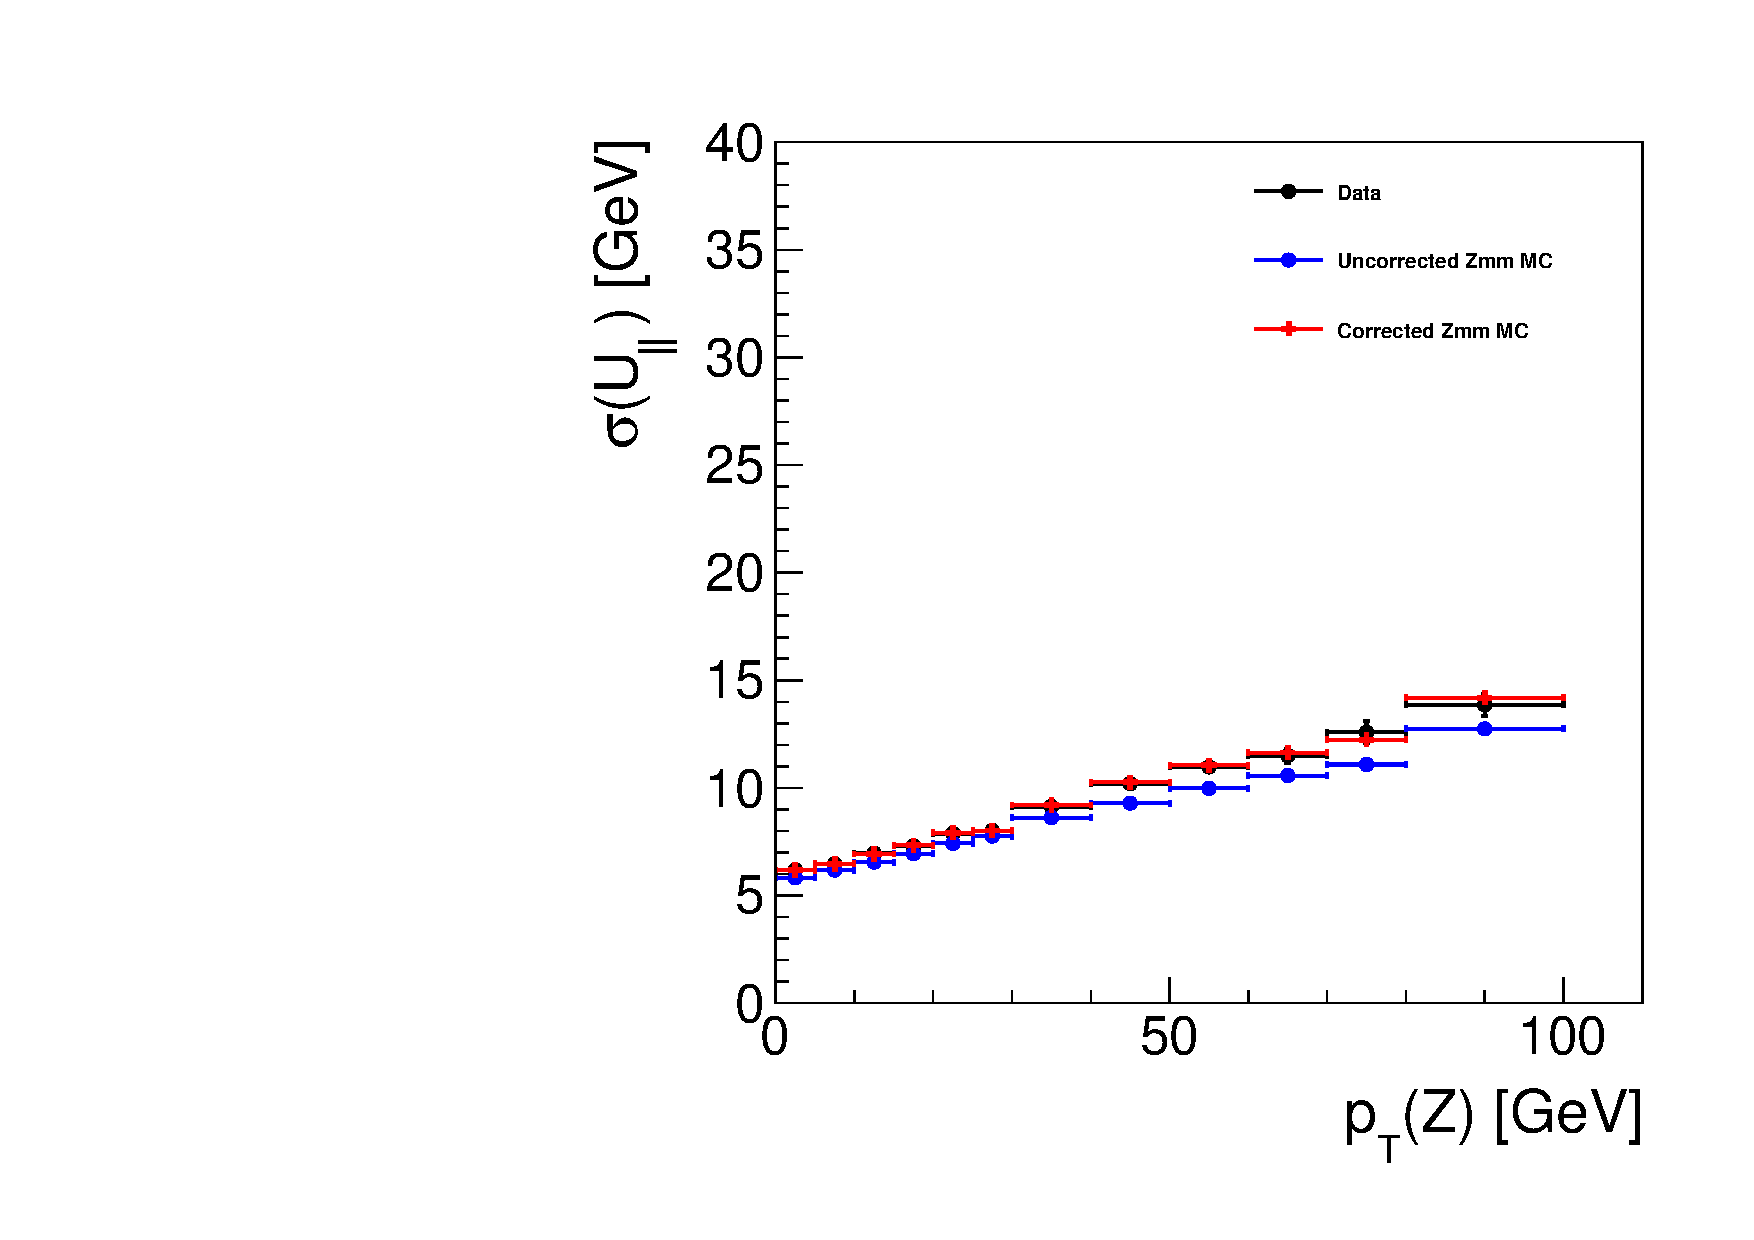
\includegraphics[width=\linewidth]{plots/Recoil/validation_5/resolution_par.pdf}
 \caption{Resolution of \upar}
%   \label{fig:Eff:el:5TeV:GSFSel:pos
\end{subfigure}%
\centering
\begin{subfigure}{.50\textwidth}
\centering
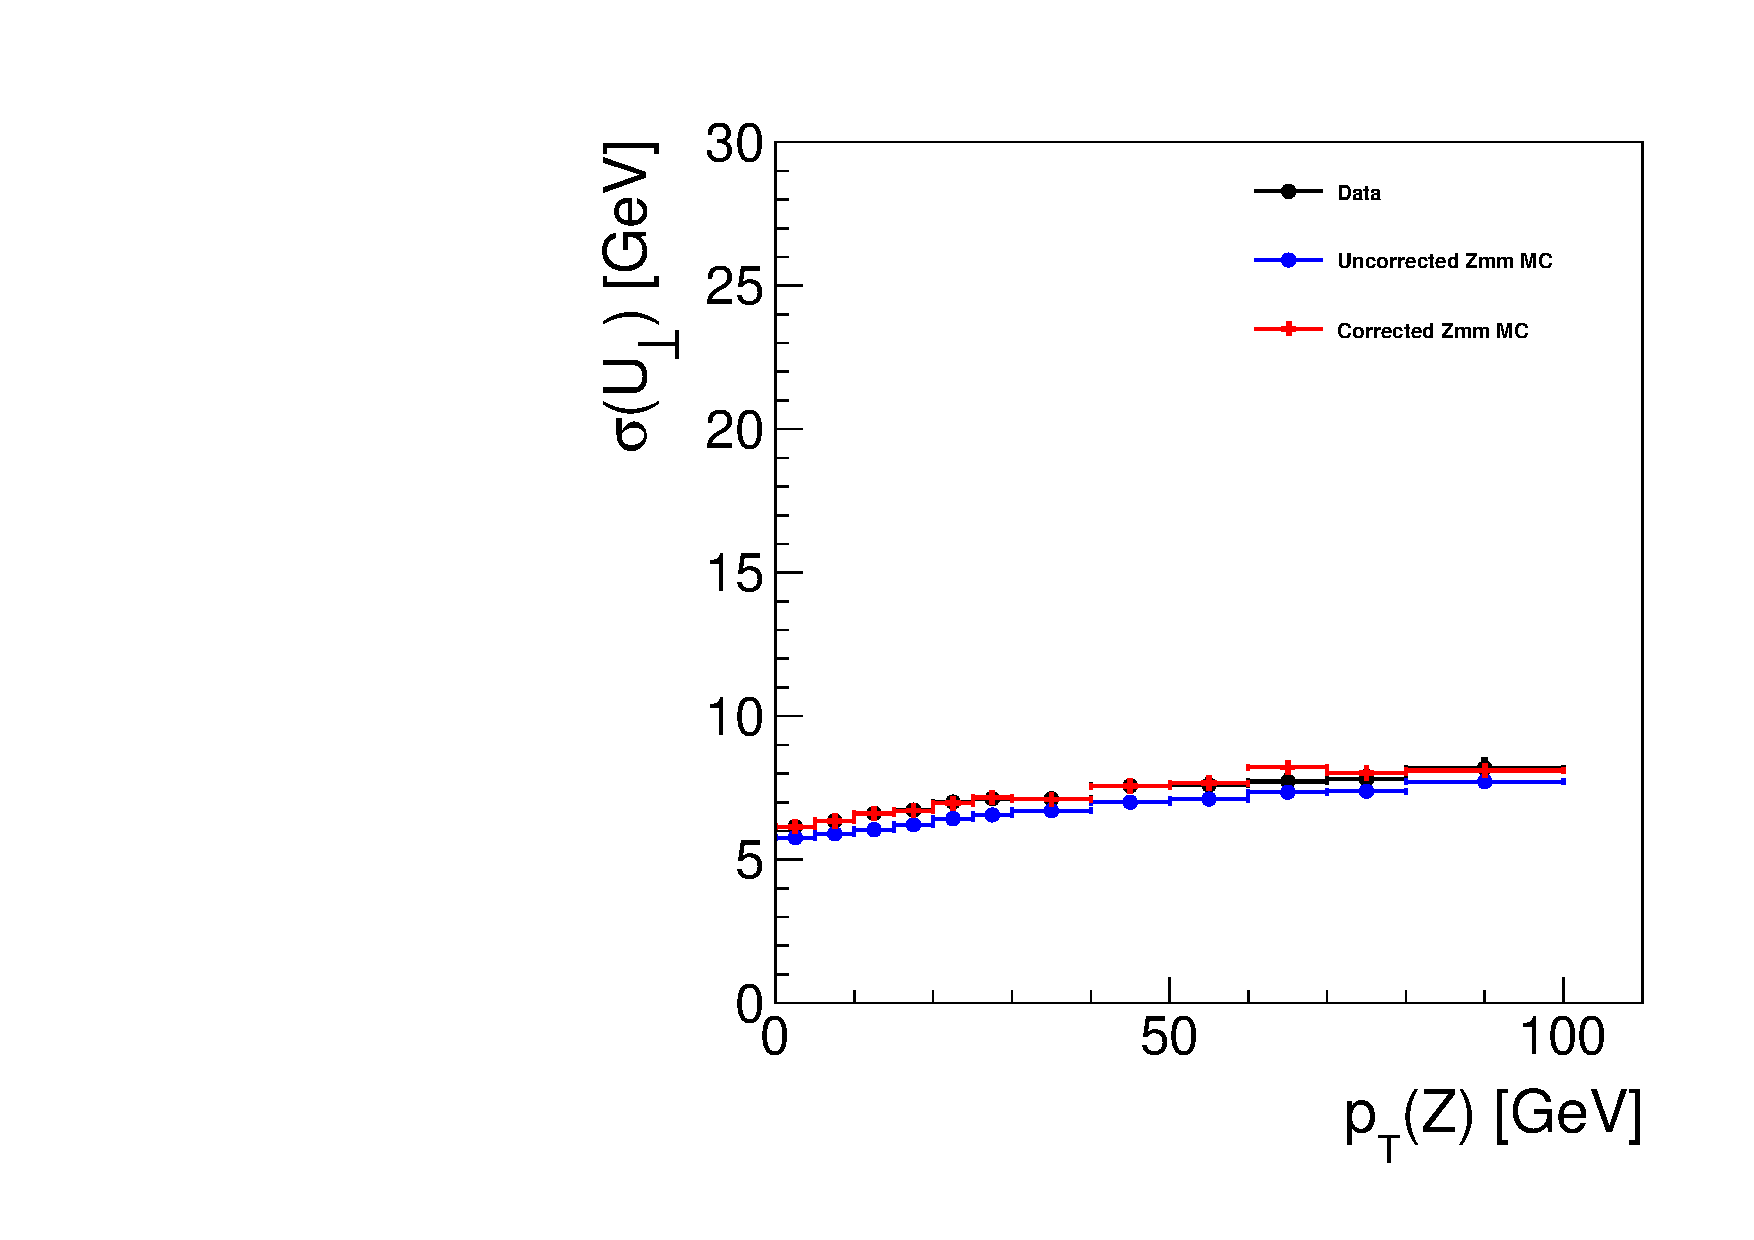
\includegraphics[width=\linewidth]{plots/Recoil/validation_5/resolution_prp.pdf}
\caption{Resolution of \uprp}
%   \caption{1a}
%   \label{fig:Eff:el:5TeV:GSFSel:pos
\end{subfigure}%
\\
\centering
\begin{subfigure}{.50\textwidth}
\centering
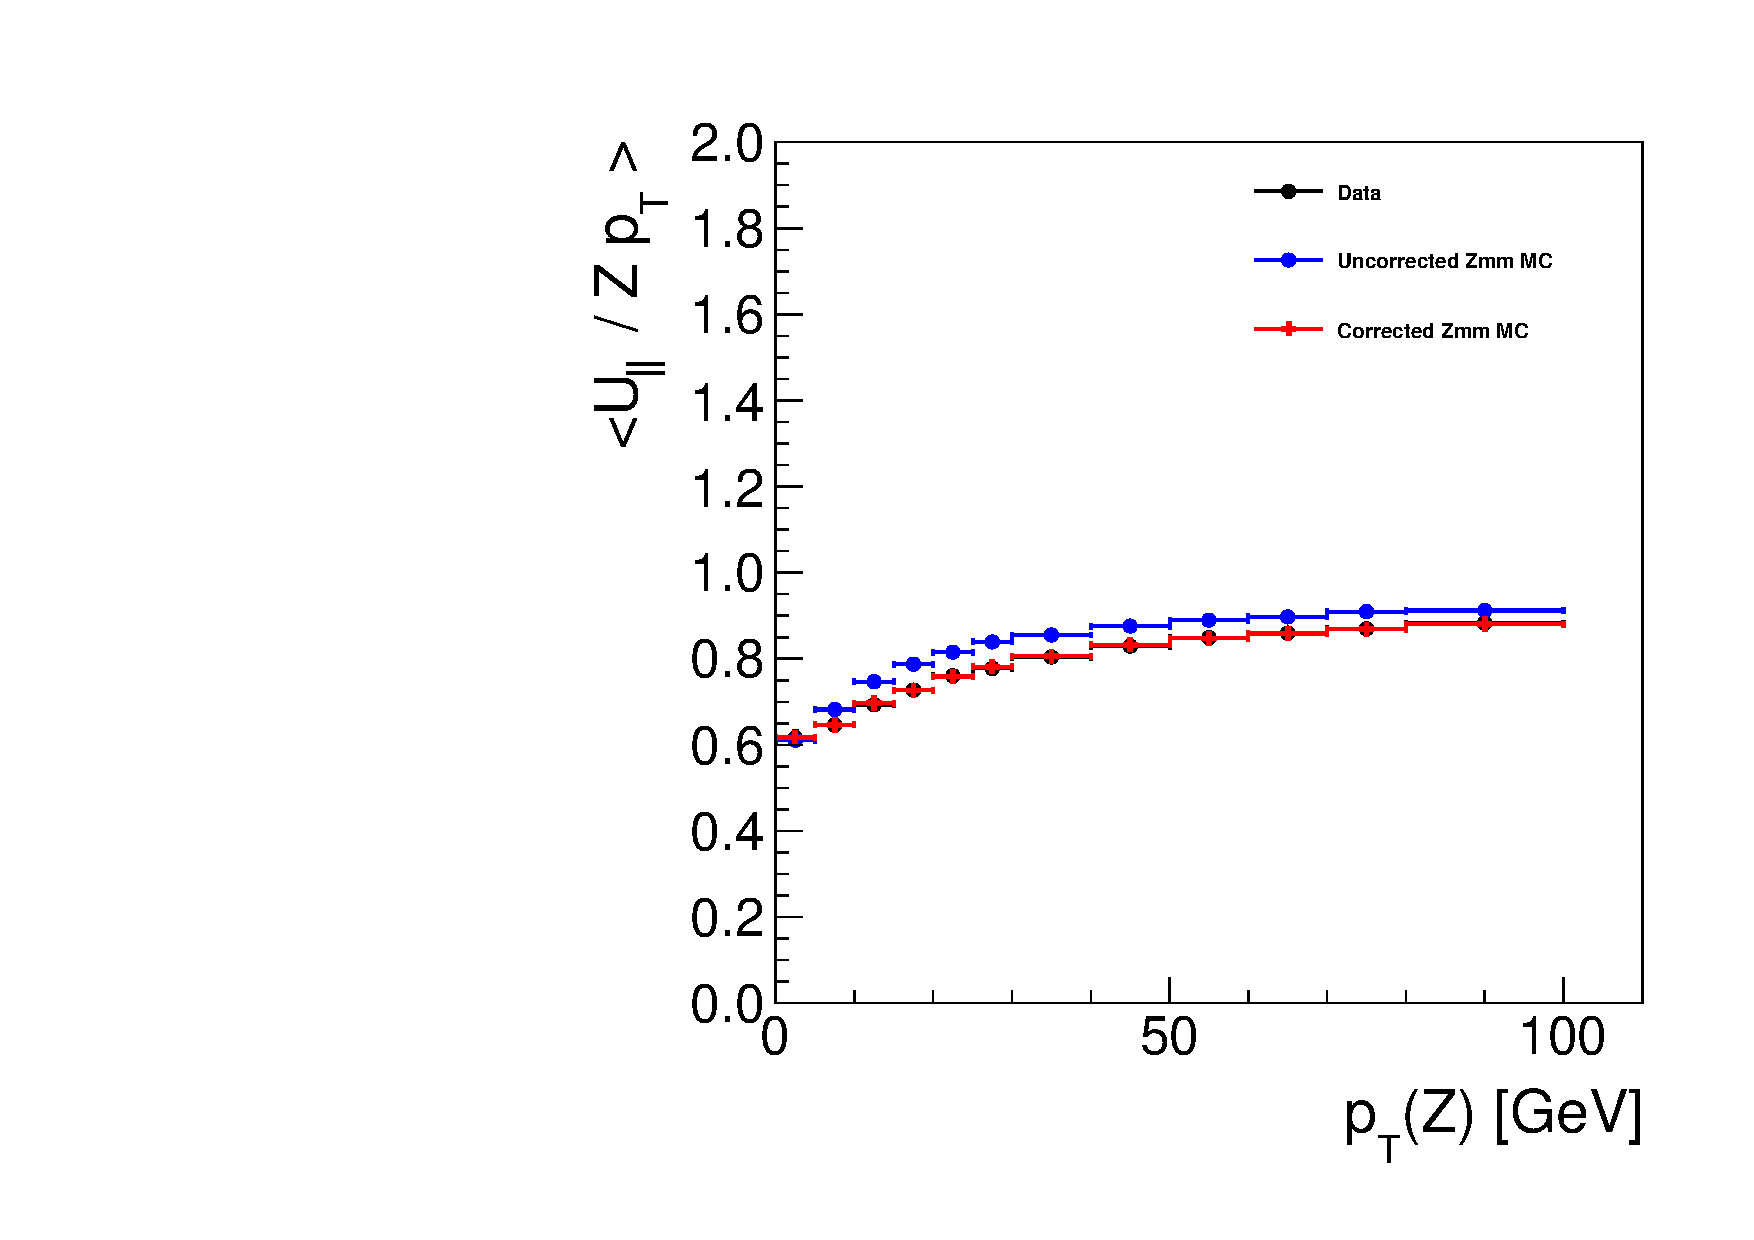
\includegraphics[width=\linewidth]{plots/Recoil/validation_5/response_par.pdf}
\caption{$p_T$-corrected response of \upar}
%   \caption{1a}
%   \label{fig:Eff:el:5TeV:GSFSel:pos
\end{subfigure}%
\caption{Closure of the recoil corrections derived from and applied to $Z\rightarrow\mu\mu$ samples for the 5 TeV dataset. The raw recoil distribution in Monte Carlo (blue) is corrected (red) towards the target spectrum of data (black).}
\label{fig:recoil:validation:5}
\end{figure}



%%%%%%%%%%%%%%%%%%%%%%%%%%%%%%%%%%%%%%%%%
%%%%%%%%%%%    Sysstematics
%%%%%%%%%%%%%%%%%%%%%%%%%%%%%%%%%%%%%%%%%

\section{Uncertainties}\label{ch:recoil:unc}
The parametrization method described above implicitly makes the assumption that the recoil distribution can uniformly be described by a double-Gaussian over the entire \pt range as well as the assumption that the parametrization can be treated as one inclusive rapidity region. Alternative models are used to address the systematic uncertainty due to these assumptions. 

The impact of these uncertainties is accounted for by propagating the differences in \met through \mt to as uncertainties on the W yield extraction fit. Additionally, statistical uncertainties for each of the fit parameters is propagated to the final result in the same way.
The details of how each of the uncertainties is calculated is listed below.
\begin{enumerate}
    \item Statistical uncertainty: covariance matrix for individual bin fit results are diagonalized. There is one eigenvalue per nuisance parameter Each eigenvalue is modified by 1$\sigma$, and new PDFs are constructed from the modified covariance matrix. The modified PDFs are then used as described in Section~\ref{ch10:recoil:apply}. 
    \item Systematic due to assumption of double-Gaussian function: A Gaussian kernel function is chosen as an alternative fitting model. 
    \item Systematic due to rapidity binning: The main correction set is binned inclusively in $y$. An alternative binning choice is to separate fits into 3 eta bins: $|y|<0.5$,~ $0.5 <  |y| < 1.0$, and $|y| < 1.0$ and fit with the 2-Gaussian function. 
\end{enumerate}
 
The difference between \met spectra from each of the listed configurations is incorporated as an uncertainty on the W signal shape in the W signal extraction fit.